\section{Аналитическая часть}

В данном разделе проведён анализ предметной области, описана структура рабочей программы дисциплины, проведена классификация баз данных (БД) и систем управления базами данных (СУБД). Рассмотрен механизм кэшированных данных, описаны возможные проблемы при его использовании и представлены методы их решения.

\subsection{Анализ предметной области}

Каждая дисциплина, преподаваемая в высшем учебном заведении, имеет свою рабочую программу. В ней хранится различная информация о дисциплине: стандарт, содержание, учебные работы, результаты обучения, перечень литературы, методические указания и прочее. Зачастую, у пользователей нет никаких автоматизированных инструментов для анализа и редактирования таких программ.

Дисциплина имеет свой федеральный государственный образовательный стандарт (ФГОС): 3+, 3++ и другие \cite{standard}. Образовательный стандарт -- совокупность обязательных требований к образованию определённого уровня и (или) к профессии, специальности. Каждый образовательный стандарт для каждого направления подготовки обучаемого имеет свою компетенцию. Компетенция содержит информацию о том, что должен знать, уметь и какими навыками должен обладать выпускник, успешно освоивший дисциплину. 

Каждому направлению подготовки, но одной и той же рабочей программы дисциплины, сопоставлены компетенции, различные в каждом образовательном стандарте. Коды компетенций для каждого образовательного стандарта отличаются.

Далее будет рассмотрена рабочая программа дисциплины <<Информатика>>, соответствующая образовательному стандарту 3++, разработанная и преподаваемая в МГТУ им. Н. Э. Баумана \cite{bmstu}.

\subsection{Структура рабочей программы дисциплины} \label{sec:rpd-structure}

Структура файлов рабочих программ дисциплин для каждого вуза может отличаться, но внутри одного вуза, скорее всего, программы имеют одну и ту же (или схожую) структуру. Рабочая программа дисциплины <<Информатика>> содержит следующие разделы:

\begin{enumerate}
	\item титульный лист;
	\item планируемые результаты обучения по дисциплине, соотнесённые с планируемыми результатами освоения образовательной программы;
	\item место дисциплины в структуре образовательной программы;
	\item объём дисциплины;
	\item содержание дисциплины;
	\item учебно-методическое обеспечение самостоятельной работы;
	\item фонд оценочных средств для проведения текущего контроля и промежуточной аттестации студентов;
	\item перечень основной и дополнительной литературы;
	\item методические указания;
	\item перечень информационных технологий;
	\item описание материально-технической базы.
\end{enumerate}

Разделы №2, №4, №5 представлены в виде совокупности текстовой информации и таблиц (рис. \ref{img:rpd_example_01}), остальные разделы представлены в виде текстовой информации (рис. \ref{img:rpd_example_02}).
\clearpage

\begin{figure}[h!]
	\begin{center}
		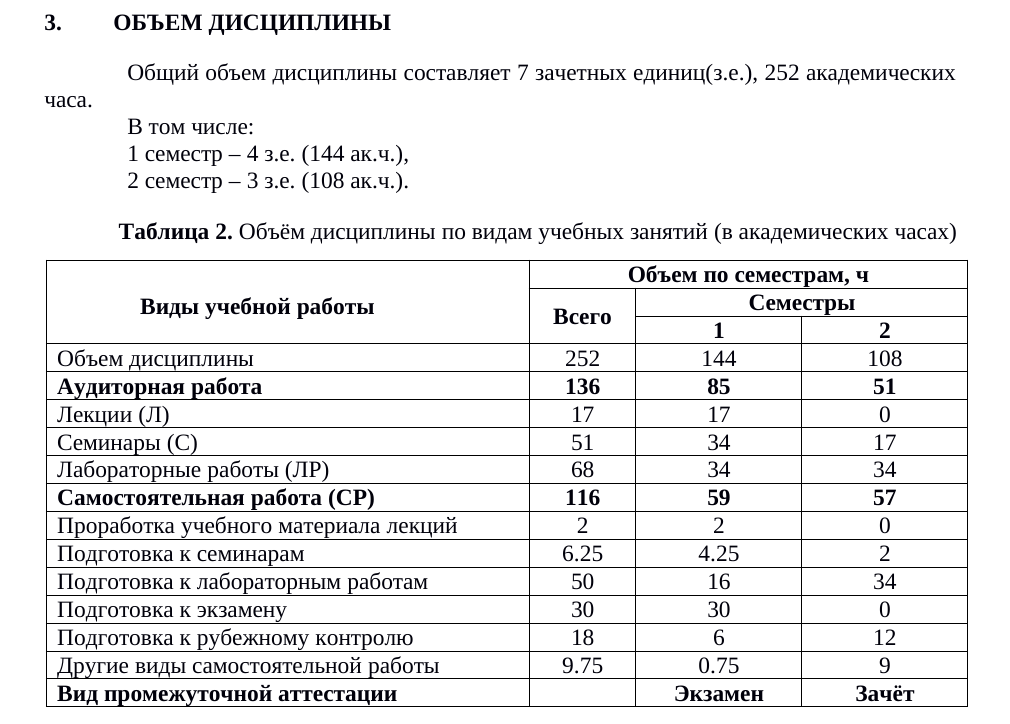
\includegraphics[scale=0.48]{inc/img/rpd_example_02.png}
	\end{center}
	\captionsetup{justification=centering}
	\caption{Изображение таблицы c информацией о объёме дисциплины.}
	\label{img:rpd_example_01}
\end{figure}

Первый раздел содержит общую информацию о курсе: название, образовательный стандарт и прочее. 

\clearpage

\begin{figure}[h!]
	\begin{center}
		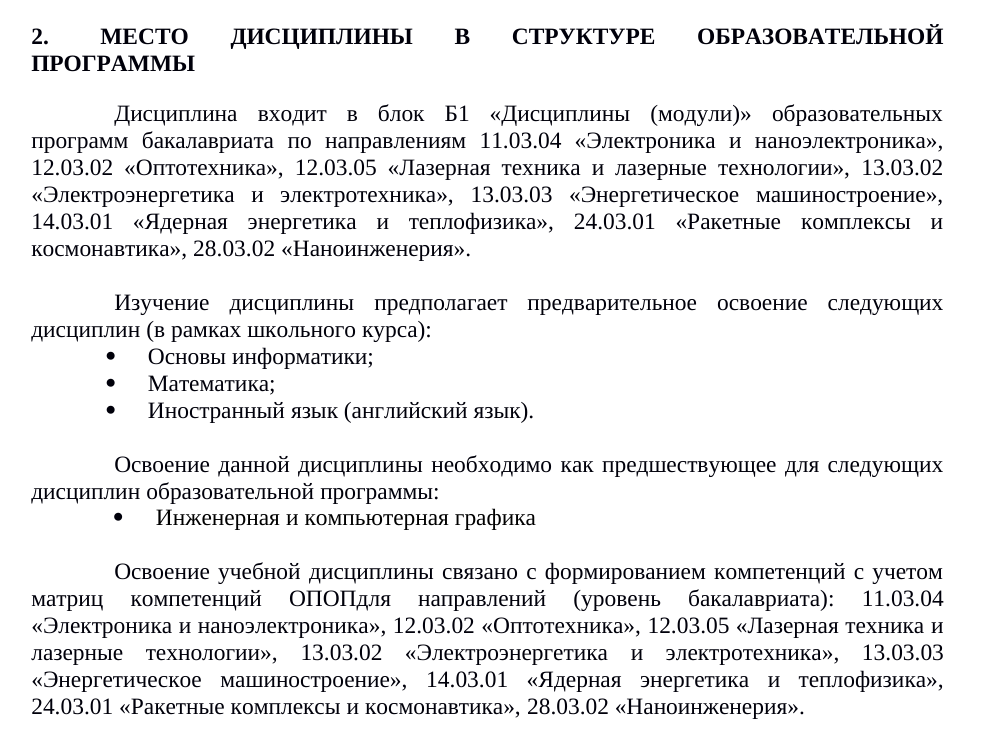
\includegraphics[scale=0.48]{inc/img/rpd_example_01.png}
	\end{center}
	\captionsetup{justification=centering}
	\caption{Изображение текстовой информации о месте дисциплине в структуре образовательной программы.}
	\label{img:rpd_example_02}
\end{figure}

Раздел №2 содержит коды и описания компетенций для каждого направления подготовки. В разделах №4 и №5 хранится информация о нагрузке и структуре дисциплины.

\subsection{Базы данных и системы управления базами данных}

Для персистентного хранения данных используются базы данных \cite{database}, контролируемые системами управления базами данных \cite{subd}.

\subsubsection{Классификация реляционных баз данных по способу хранения}

Реляционные базы данных по способу хранения делятся на две группы: строковые и колоночные.\\

\noindent\textbf{Строковые базы данных}

Строковыми базами данных называются такие базы данных, записи которых хранятся построчно, в основном такой тип используется в транзакционных системах (англ. \texttt{OLTP} \cite{OLTP}), для которых характерно большое количество коротких транзакций с операциями вставки, обновления и удаления данных. Системы OLTP наиболее подходят для быстрой обработки запросов и поддержания целостности данных в средах с множественным доступом.\\

\noindent\textbf{Колоночные базы данных}

Колоночными называются базы данных, записи которых хранятся по \\* столбцам, в основном такой тип используется в аналитических системах (англ. \texttt{OLAP} \cite{olap}), которые характеризуются низким объёмом транзакций, а запросы часто являются составными и включают в себя агрегацию, мерой эффективности таких систем является время отклика. Наличие агрегированных и исторических данных позволяет использовать OLAP-системы для реализации методов интеллектуального анализа.

\subsection{Кэширование данных}

Чтобы уменьшить время отклика, можно использовать механизм кэширования данных, для реализации которого подходят \texttt{NoSQL} \cite{nosql} \texttt{in-memory} базы данных, хранящие данные в оперативной памяти, что обеспечивает более быстрый доступ, по сравнению с традиционными реализациями.

\subsubsection{Проблемы кэширования данных}

\noindent\textbf{Проблема синхронизации данных}

Приложение пишет в кэш и базу данных, которые между собой никак не синхронизируются, таким образом возникает несогласованность данных. Например, возможна ситуация, когда данные удаляются из хранилища и их нужно удалить из кэша. Эту проблему можно решить установкой триггеров, которые будут срабатывать на изменение и удаление записей, чтобы синхронизировать данные в кэше.

\noindent\textbf{Проблема <<холодного старта>>}

Когда кэш только создаётся, он пуст и не имеет никаких данных -- все запросы идут напрямую в БД, и только через некоторое время кэш будет содержать необходимую информацию. Эту проблему можно решить, выбрав СУБД с журналированием всех операций -- при перезагрузке можно восстановить предыдущее состояние кэша с помощью журнала событий, который хранится на диске. При перезагрузке кэша нужно синхронизировать данные с хранилищем -- возможно, какие-то данные, находящиеся в кэше, перестали быть актуальными за время его перезагрузки.
